\documentclass{beamer}
\usetheme{Boadilla}
\title{Language Processor Introduction 1}
\subtitle{Dr. C\'esar Ignacio Garc\'{\i}a Osorio \\ \href{mailto:cgosorio@ubu.es}{cgosorio@ubu.es}}
\author{Cao, Thi Huyen(Lilli-L3I2) \\ \href{mailto:caothivananh98@gmail.com}{caothivananh98@gmail.com}}
\institute{University of Burgos}
\date{\today}


\begin{document}


\begin{frame}
\titlepage
\end{frame}


\begin{frame}
\frametitle{Introduction to Language Processor}
\begin{center}
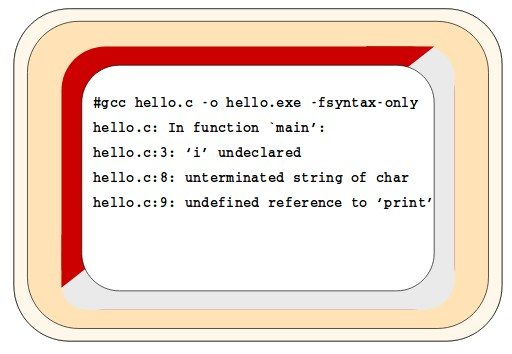
\includegraphics[scale=0.5]{1}
\end{center}
\end{frame}


\begin{frame}
\frametitle{Language Processor}
\begin{block}{Definition}
A language processor is a computer program, which takes a sequence of characters (some kind of text in a language) as an input, analyses it, optimizes some processes and returns a result
\end{block}
Emilio Vivancos
Rubio, Universidad Politécnica de Valencia
\href{https://www.youtube.com/watch?v=aT5EGLgJs88/}{\underline{https://www.youtube.com/watch?v=aT5EGLgJs88}}
\end{frame}


\begin{frame}
\frametitle{Compiler}
\begin{block}{Definition}
A compiler is a program, which translates a program called source program, which is written in a language called source language into a target program of target language. In addition a compiler emits some error messages
\end{block}
\begin{center}
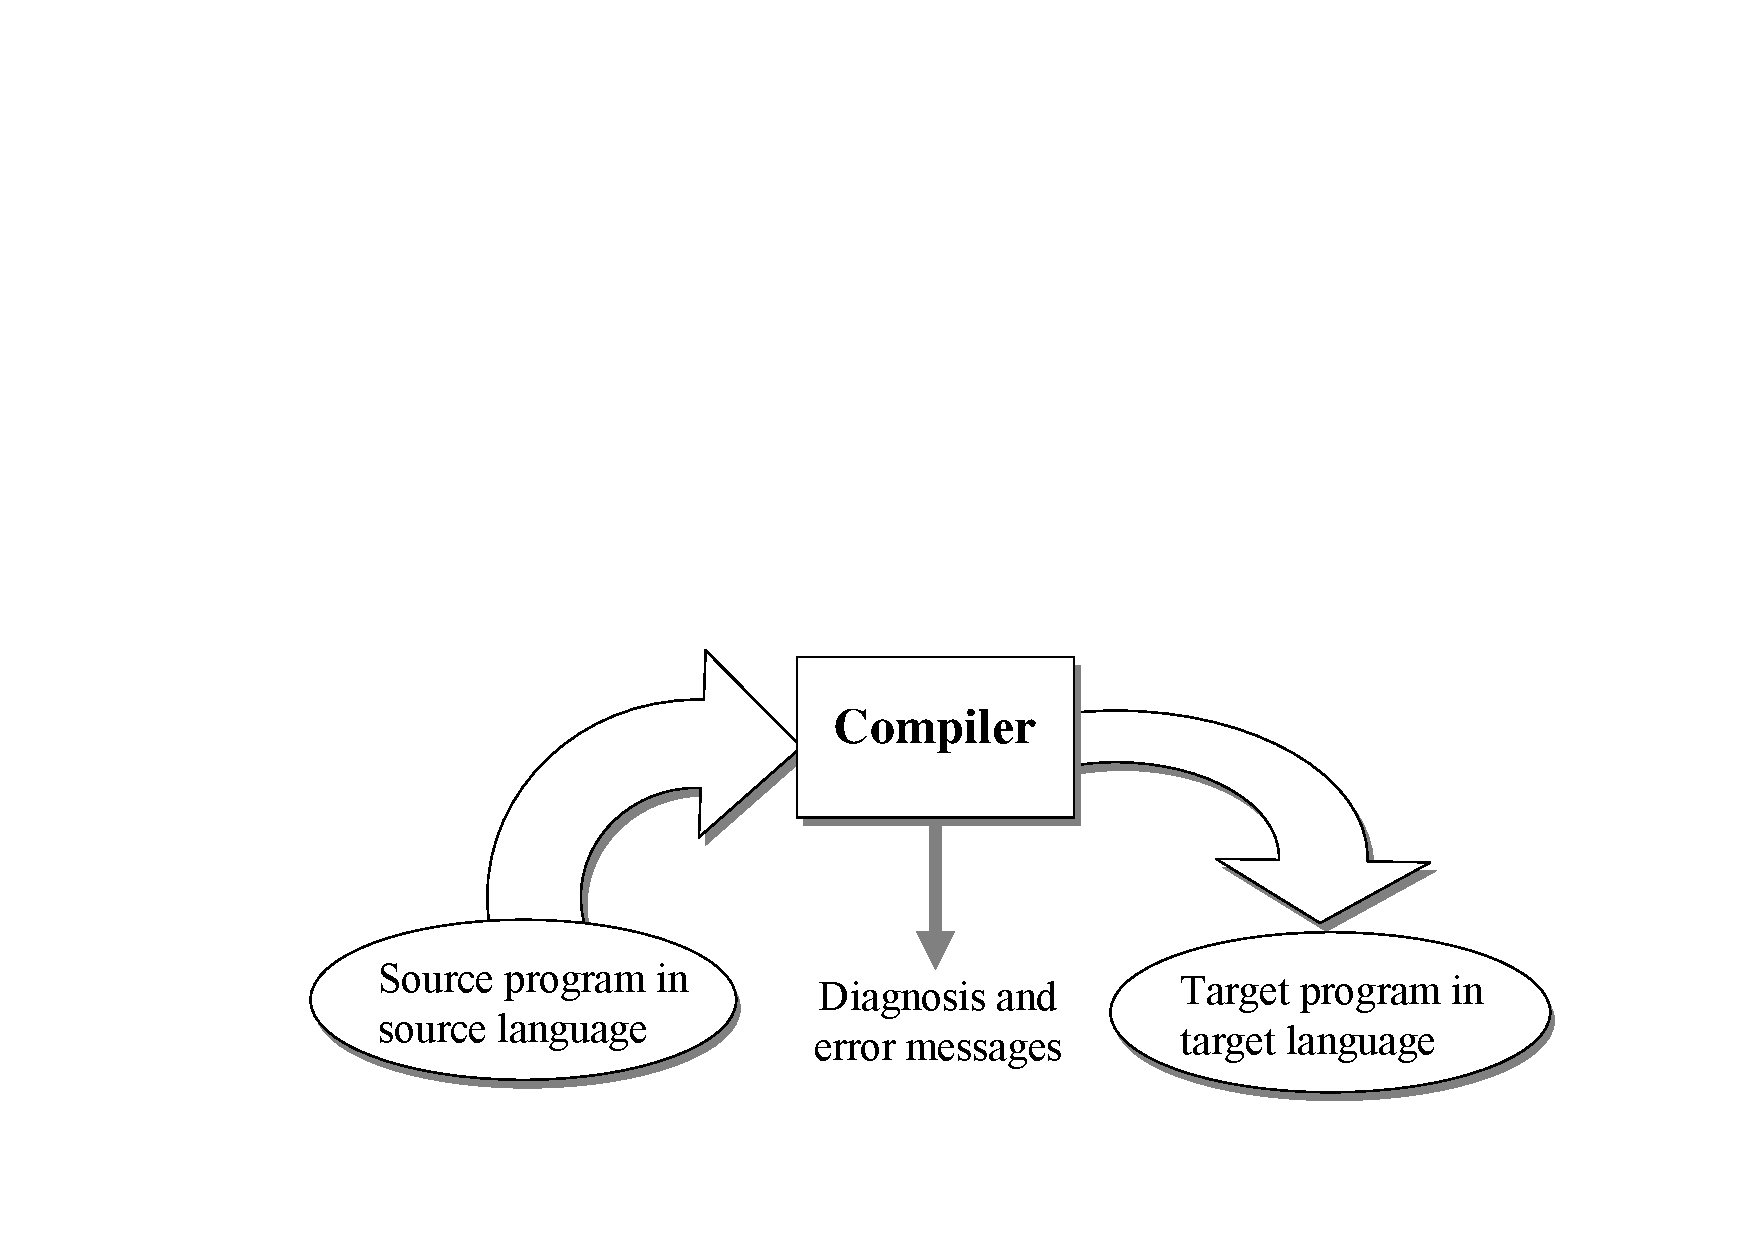
\includegraphics[scale=0.5]{2}
\end{center}
\end{frame}


\begin{frame}
\frametitle{Field of use 1}
\begin{block}{Usage}
Compiler building techniques are used in many different fields
\end{block}
\begin{itemize}
\item The editor of highlighted syntax makes it easy to edit the program
\item The program for text formatting( for example TeX, LaTeX, which from the documentation and formatting commands allows obtaining a suitable file for visualization or printout 
\item Static syntax checker( such as lint) allows detection of many errors before compilation (something similar to option \textbf{-fsyntax-only} of GNU gcc Compiler
\item The intepreters (for language like Lisp or Basic, or for programs with their own interpretation languages such as Derive or Mathematics
\item Macro languages of extensible applications(Scheme in the world of GNU and Visual Basic for applications in the world of Microsoft Windows)
\end{itemize}
\end{frame}


\begin{frame}
\frametitle{Field of use 2}
\begin{itemize}
\item Script languages and ``glue'' languages ( perl, tcl/tk, python) allows rapid development of applications with parts written in different languages
\item Analyse of configuration file requires in a lot of modern systems( file .ini of Microsoft Window or source files of X)
\item Silicon circuit compiler (for special languages, which describe the layout of printed circuit, obtain the mask for getting the circuit through photographic techniques
\item Query languages for databases
\item Analyse of protocol specifications for communicating in specified formal languages ( such as \href{https://en.wikipedia.org/wiki/Abstract_Syntax_Notation_One}{\underline{Abstract Syntax Notation}}-ASN.1)
\item Translation of \href{https://en.wikipedia.org/wiki/JavaServer_Pages}{\underline{JSP}} pages to \href{https://en.wikipedia.org/wiki/Java_serlets}{\underline{Servlets Java}} 
\item \href{}{\underline{Google Web Toolkit}}(Java-Javascript translator)
\item Translation of style sheet \href{https://es.wikipedia.org/wiki/LESS_(lenguaje_de_hojas_de_estilo)}{\underline{LESS}} \href{https://es.wikipedia.org/wiki/Sass_(lenguaje_de_hojas_de_estilo)}{\underline{SASS}}
\href{https://en.wikipedia.org/wiki/Cascading_Style_Sheets}{\underline{CSS}}
\end{itemize}
\end{frame}


\begin{frame}
\frametitle{Field of use 3}
\begin{itemize}
\item Preprocessor modifies source text in a certain format before compiling ( many compilers support macro instructions beyond the language itself, which tells the compiler to include an external file to complete compilation list (Qt, gcc -E)
\item Translation of natural language like translation from a natural language to another. For example Spanish to English (There is no achievement currently fundamentally due to the ambiguity of natural language. The greatest achievements in this field is work with a subset of natural language, limit valid syntax construction and/or vacabulary. This topic is usually mentioned in artificial intelligence techniques)
\item Bioinformatics Grammars are used to defined languages and more precise grammar are used to model the structure of RNA sequences
\end{itemize}
\end{frame}


\begin{frame}
\frametitle{A small view of history 1}
\begin{itemize}
\item
\item
\item
\end{itemize}
\end{frame}


\begin{frame}
\frametitle{A small view of history 2}
\begin{itemize}
\item
\end{itemize}
\end{frame}


\begin{frame}
\frametitle{A small view of history 3}
\begin{itemize}
\item
\begin{itemize}
\item
\end{itemize}
\end{itemize}
\end{frame}


\begin{frame}
\frametitle{A small view of history 4}
\begin{itemize}
\item
\end{itemize}
\end{frame}


\begin{frame}
\frametitle{Use of high level languages}
\begin{block}{Information}
Compiler of high-level languages are currently well established
\end{block}
\begin{table}
\begin{tabular}{|c|c|}
\hline
Advantage & Disadvantage\\
\hline
Improving programmer's productivity& Slower than assembler\\
\hline
Reduction of logical errors& big programs\\
\hline
Easy to clean &\\
\hline
\end{tabular}
\end{table}
\end{frame}


\begin{frame}
\frametitle{Intepreter vs Compiler}
\begin{itemize}
\item There are two ways to run a program written in high-level languages
\begin{itemize}
\item Compiler: translating the entire program to another equivalent program in machine code. That program is execuatble
\item Interpreter: interpreting program instructions written in high-level language and executing them one by one
\end{itemize}
\end{itemize}

\begin{table}
\begin{tabular}{|p{5cm}|p{5cm}|}
\hline
Interpreter & Compiler \\
\hline
Easy to locate errors&Dificult to locate errors\\
\hline
Every time the program is executed, its interpretation is necessary& Only one compilation is necessary. After it's done, the execution speed is high\\
\hline
Sufficient in developing and debugging& Sufficient when there is no more error (exploitation)\\
\hline
\end{tabular}
\end{table}
\end{frame}


\begin{frame}
\frametitle{Structure of a compiler 1}
\begin{center}
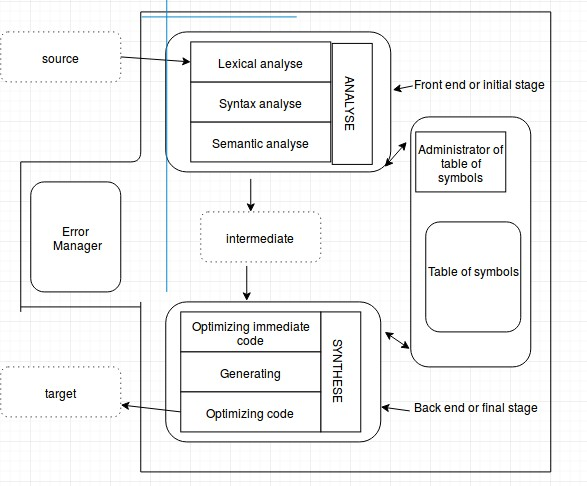
\includegraphics[scale=0.5]{3}
\end{center}
\end{frame}


\begin{frame}
\frametitle{Structure of a compiler 2}
The compilation process can be divided into some phases, which simultaneously or consecutively transforms the source program from one represtation to another.
\begin{block}{Information}
In practice, some phases can be grouped together and temporatory representations between the groups don't need to be built explicitly
\end{block}
\textbf{front end }= lexical + syntax + semantic\\
(\textbf{middle end} = generation of intermediate code\\
\textbf{back end} = opt. intermediate code + gen. code + opt. code\\
\end{frame}


\begin{frame}
\frametitle{Structure of a compiler 3}
The front-end(analysis or intitial stage) depends mainly on the source language, is designed properly. It's possible to use different back-end(synthesis or final stage) because it includes the phrases, which depend on the target machines. So that the code can be run in different machines
\end{frame}


\begin{frame}
\frametitle{Analyse}
\end{frame}
\begin{frame}
\frametitle{Synthese}
\end{frame}
\begin{frame}
\frametitle{Error manager}
A compiler has to have a certain behavior against erroneous programs. This process is grouped in a phase called error handler. Each of the previous phases interacts with the error manager
\end{frame}
\begin{frame}
\frametitle{Table of symbols manager}
\end{frame}


\begin{frame}
\frametitle{Compiling process 1}
\begin{center}
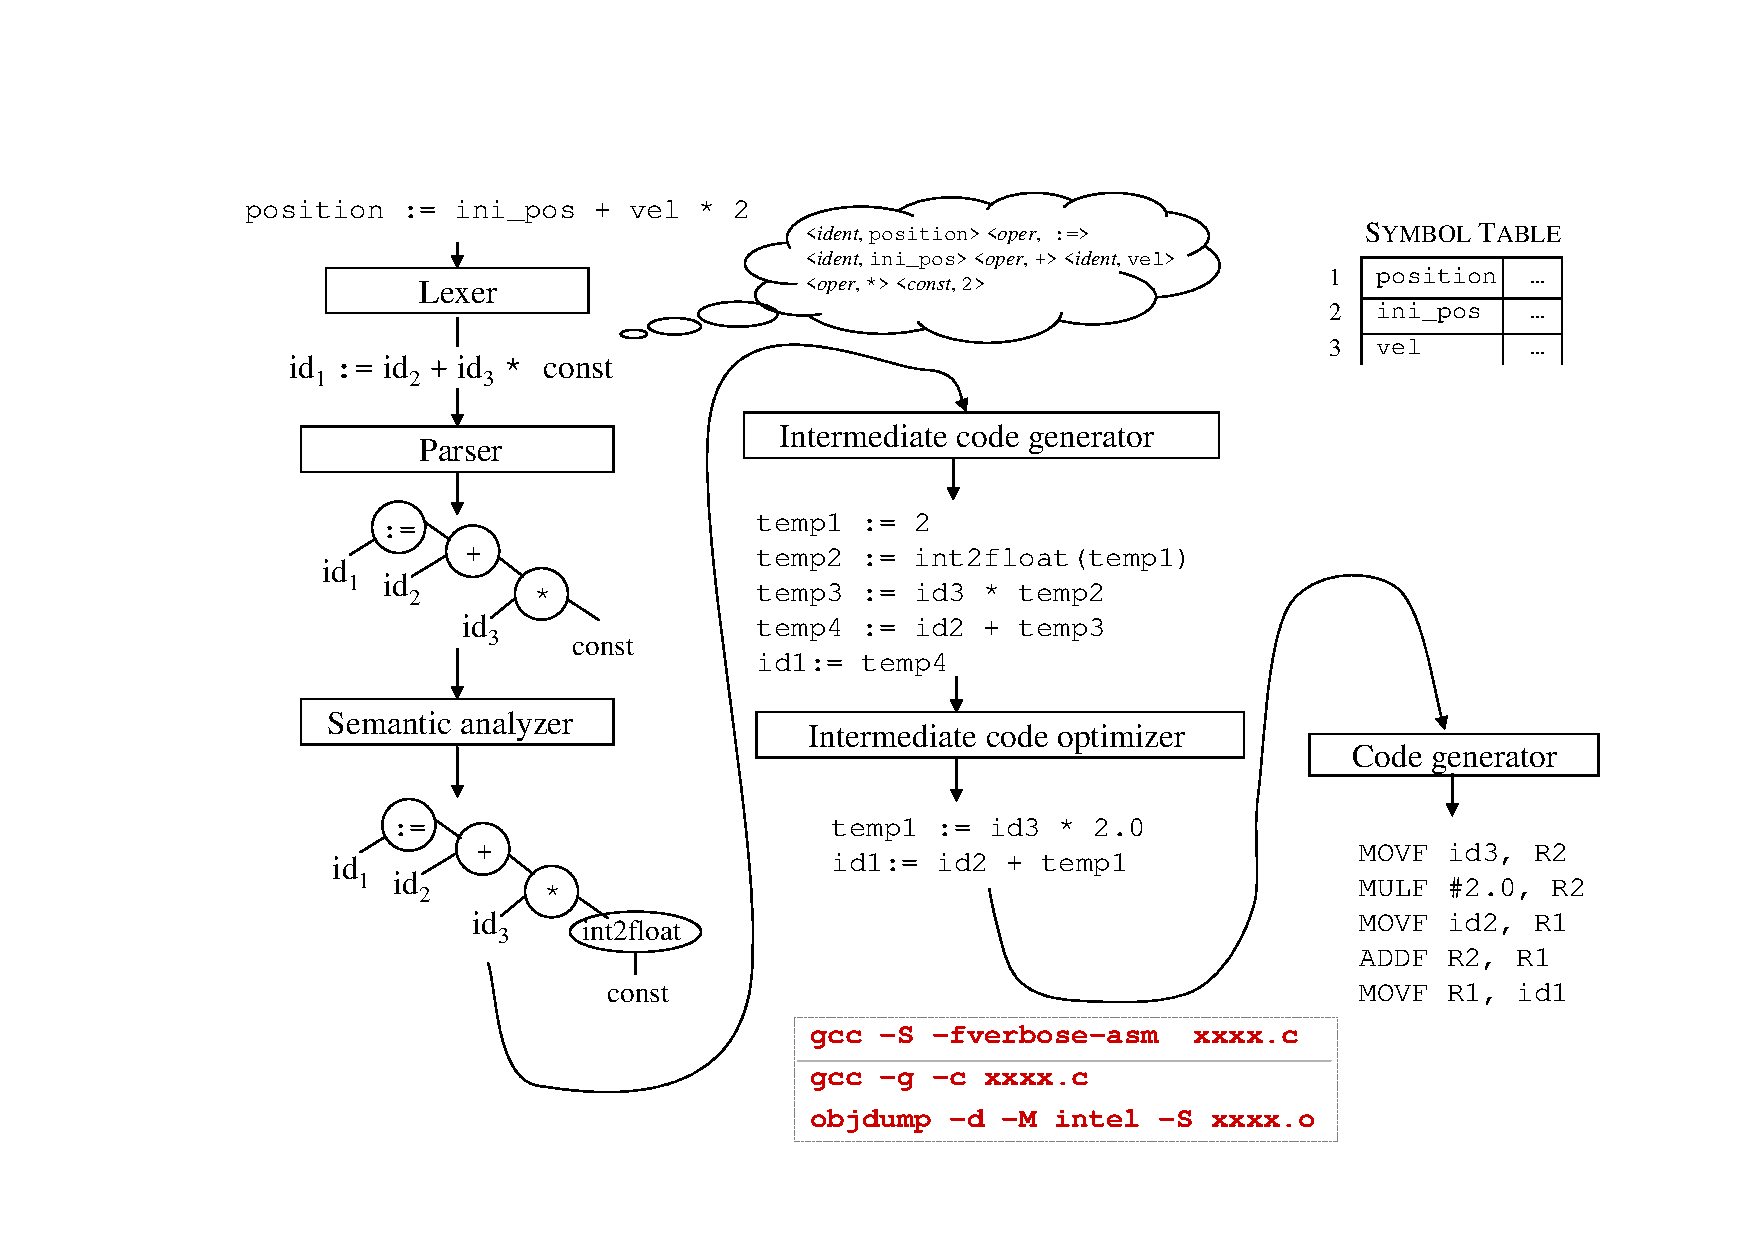
\includegraphics[scale=0.48]{5}
\end{center}
%analizador lexico: lexical analyser,analizador sentactico: syntax analyser,analizador semantico: semantic analyser\\
%Generador de código intermedio: intermediate code generator\\
%optimizador de código intermedio: intermediate code optimizer\\
%Generador de código: code generator\\
\end{frame}


\begin{frame}
\frametitle{Working environment of a compiler}
\begin{center}
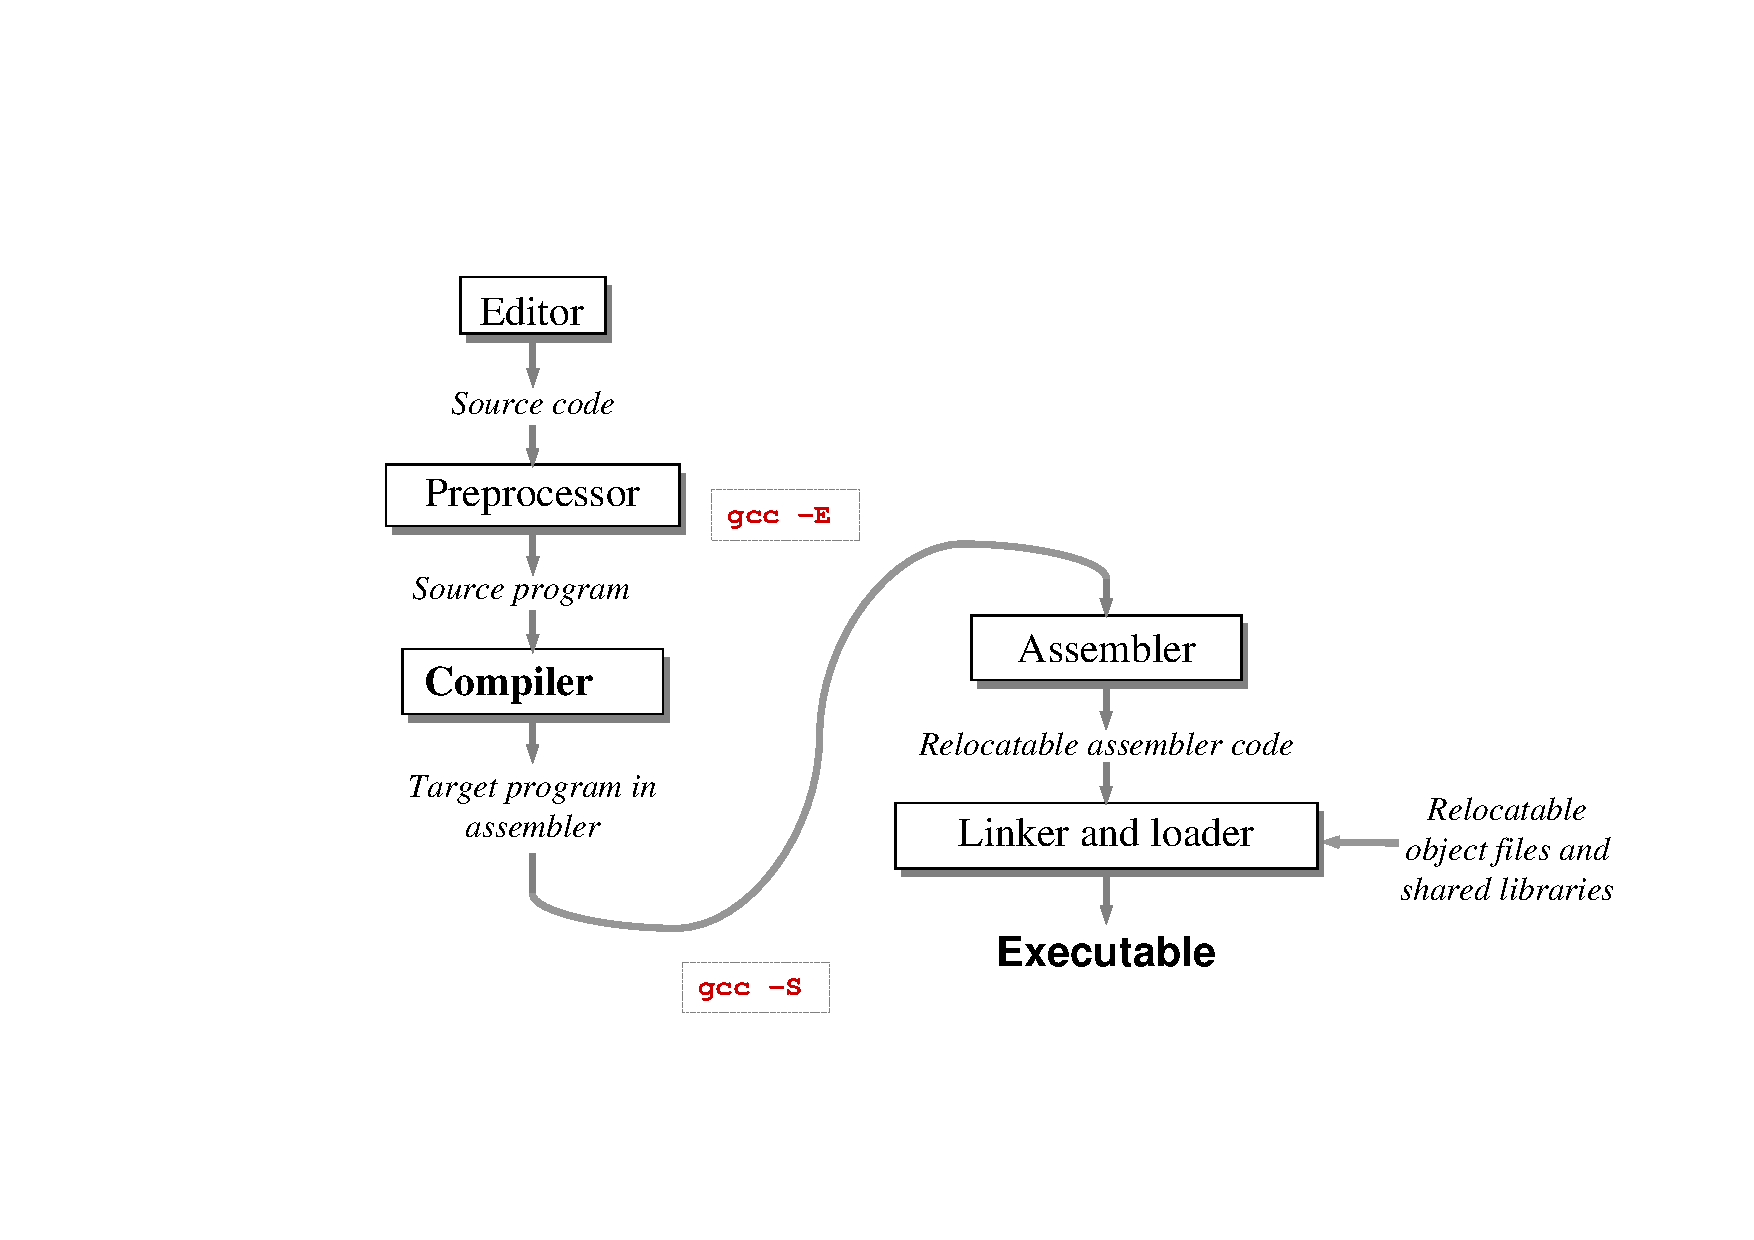
\includegraphics[scale=0.5]{4}
\end{center}
\end{frame}


\begin{frame}
\frametitle{Consruction of a compiler}
In building a compiler, there are several approaches, which are:
\begin{itemize}
\item in assembler: efficient compilers but difficult to maintain
\item in a high-levellanguage: easy to maintain but requires a lot of development time
\item using compiler building tools like Flex, Bison, JavaCC, JJTree, JTB
\end{itemize}
\end{frame}


\begin{frame}
\frametitle{Tools}
\begin{itemize}
\item Generators of syntax analyzer
\begin{itemize}
\item Generate syntactic analyzers based on context-independent grammar (eg, yacc, bison, JavaCC, ANTLR)
\end{itemize}
\item Generators of lexical analyzers
\begin{itemize}
\item Generate automatically lexical analyzers based on a specification based on regular expressions (eg lex, flex, JavaCC, ANTLR)
\end{itemize}
\item Generators of tree syntax
\begin{itemize}
\item Making it easy to create tree syntax(JJTree, JTB)
\end{itemize}
\end{itemize}
\end{frame}


\begin{frame}
\frametitle{Tools}
\begin{itemize}
\item Syntax-Directed Translation Devices
\begin{itemize}
\item Providing groups of routines, which run through the tree and generating intermediate code
\end{itemize}
\item Automatic code generators
\begin{itemize}
\item Taking a set of rules, which define the translation from intermediate language to machine language. The fundamental technique is matching template
\end{itemize}
\item Devices for data flow analysis
\begin{itemize}
\item Allowing code optimization based on a collection of information about how important that part is while transmitting one to another
\end{itemize}
\end{itemize}
\end{frame}


\begin{frame}
\frametitle{Tools}
\begin{itemize}
\item formal tools
\begin{itemize}
\item Grammar
\item Turing machine
\item derterminate and indeterminate final automat
\item Stack automat
\item Analysis LL, LR, SLR and LALR
\end{itemize}
\item programming tools
\begin{itemize}
\item Yacc/bison
\item Lex/flex/jlex
\item JavaCC, ANTLR, Lemon, Ply, SableCC, CUP...
\end{itemize}
\end{itemize}
\end{frame}


\end{document}